\chapter{Technológiák}
\label{chapTech}

\section{Docker}
\label{docker}
\paragraph{}
Kezdjük azzal, hogy meghatározzuk, mi a Docker.
Azért a Dockerrel kezdem mivel ez az alapja az egész projektemnek.
A Docker honlapja jelenleg a következőképpen határozza meg a Dockert (Szabad fordításban):

\paragraph{}
"A Docker a világ vezető szoftveres tárolóplatformja, a fejlesztők a Docker-t használják az "én gépemen működik" problémák kiküszöbölése érdekében, amikor a munkatársakkal együtt dolgoznak egy kódon. Az üzemeltetők a Dockert használják az alkalmazások futtatására és kezelésére egy szerveren elválasztva egymástól a legjobb kihasználtságért, A vállalatok a Docker-t használják agilis szoftverszállítási folyamatokhoz, hogy gyorsabbá és biztonságosabbá tegyék a Linux és a Windows Server alkalmazásaikat." \cite{dockerswebpage}

\paragraph{}
Ez egy elég merész megnyitó nyilatkozat, de ha megnézzük a Docker vezérigazgatója, Ben Golub által bemutatott számokat a 2017-es DockerCon megnyitása során, amelyek a következők:

 - 14 millió Docker fogadó
 
 - 900,000 Docker Alkalmazások
 
 - 7700 százalékos növekedés a Docker "Image"-k letöltésében
 
 - 3300 projektpartner

Egy olyan technológia esetében, amely csak három éves, mindenki egyet kell hogy értsen ez meglehetősen lenyűgöző teljesítmény.  \cite{dockercondata2017}

\subsection{Különbségek dedikált hostgépek, vitruális gépek és a Docker közt}
\label{dockerdiff}
A Docker egy konténerkezelő rendszer, amely hasonlít a Linux Containers (LXC)-re de könnyebb és univerzálisabb módon azt.
Lehetővé teszi a virtuális környezetben lévő képek létrehozását akár laptopon, ugyanis a futtatásuk nem igényel nagy erőforrást.
Ebben a környezetben a saját gépén helyi szinten futó konténeren végrehajtott műveletek vagy parancsok ugyanazok amelyeket megszokhattunk egy valódi gépen.
Ez segít abban, hogy ne kelljen másképp csinálni a dolgokat, ha egy olyan fejlesztői környezetből, mint amilyen a helyi gépen található, szerver szintű környezetébe lépünk.

\pagebreak

Nézzük meg a Docker konténerek és egy tipikus virtuális gépi környezet közötti különbségeket.
Az alábbi ábra bemutatja a dedikált, host gép és a virtuális gép közötti különbséget:

\begin{figure}[h]
	\centering
	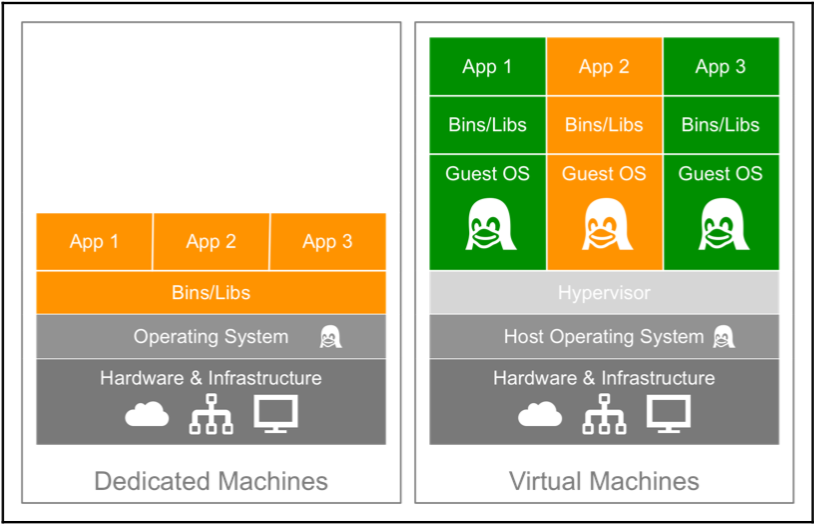
\includegraphics[width=1\linewidth]{figures/host-machine-vs-vm}
	\caption{Egy Host gép és egy Virtuális gép közti különbség}
	\label{fig:hostvsvm}
	\cite{gallagher2015mastering}
\end{figure}

\paragraph{}
Mint látható a kép bal oldalán, egy dedikált gépen három alkalmazást futtatunk, mindegyik ugyanazt a narancssárga szoftvercsomagot tartalmazza. 
Ez egy alap hardver, operációsrendszer, telepített alkalmazások és a hozzájuk tartozó csomagok rendszer.
Nehezen szabályozható, monitorozható és az erőforrás elosztást is nehezen lehet kivitelezni.
A virtuális gépek futtatása már lehetővé teszi számunkra, hogy három alkalmazást futtassunk, két teljesen más szoftvercsomaggal.
Mi szabályozhatjuk hogy a host gépből menyit adunk át a virtuális gépnek és tudjuk őket külön monitorozni.
A kép baloldalán látható hogy a host operációs rendszeren felül még 3 vendég rendszert is futtatnunk kell.
A három rendszer mellett az ábra mutatja ugyanazokat az alkalmazásokat (narancssárga és zöld), amelyek a Docker használatával egy konténerekben futnak, mivel ugyan azokat a csomagokat használják.

\pagebreak

\begin{figure}[h]
	\centering
	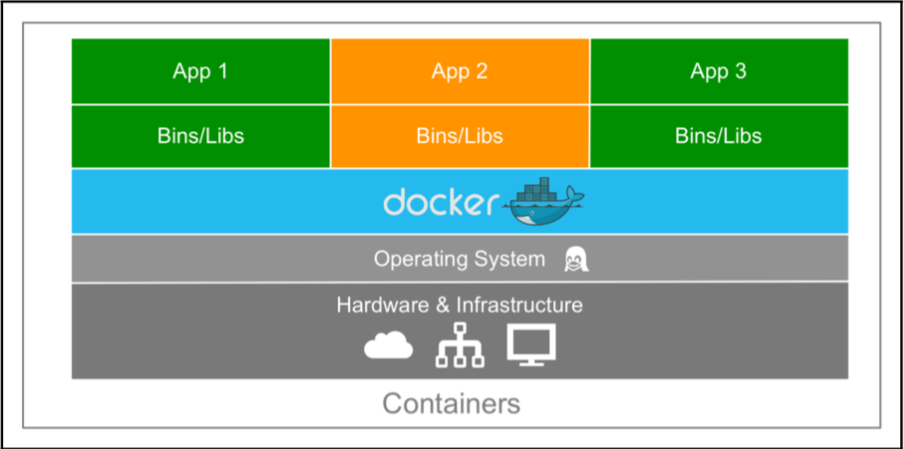
\includegraphics[width=1\linewidth]{figures/docker-work}
	\caption{Egy Dockert futtató gép és konténerei}
	\label{fig:docker-work}
	\cite{gallagher2015mastering}
\end{figure}

\paragraph{}
Ez az illusztráció nagyon jó betekintést nyújt a Docker legfontosabb előnyeibe.
Nincs szükség egy teljes operációs rendszerre minden alkalommal, amikor új konténert hozunk létre ami lecsökkenti a konténerek teljes méretét.
A Docker gazdagép Linux kernelének használatára támaszkodik, mivel a Linux szinte minden verziója a szabványos kernel modelleket használja.
%Így a Docker által épített operációs rendszerek, például a Red Hat, a CentOS és az Ubuntu számára. 
Emiatt szinte bármilyen Linux operációs rendszert futhat a gazda gép, és képes lesz a Linuxon alapuló operációs rendszerek futtatására. 
Ez igaz a Unix alapú operációs rendszerekre is, így egy macOS-el telepített host gép is képes szinte bármilyen Linux konténert futtatni (Kivételek pl.: RHEL, SLES). 
Ugyan az alkalmazások úgy látják hogy egy teljes értékű operációs rendszeren futnak, valójában csak a binálisok és csomagok például Apache, Java és könyvtáraik szükségesek az alkalmazások futtatásához.
Például a korábbi ábrán látható, hogy például a narancssárga alkalmazáshoz Red Hat, a zöld alkalmazáshoz pedig Debian szükséges.
Soha nem lesz szükség a Red Hat vagy a Debian telepítésére, így a Docker egy másik előnye a képek mérete kerül előtérbe.
A konténerek a legnagyobb darab nélkül épülnek fel azaz a rendszermag vagy az operációs rendszer nélkül.
Így rendkívül kicsi, kompakt és könnyen szállítható "konténereket" kapunk.


\pagebreak
\subsection{Maven}
\paragraph{}
Az Apache Maven népszerű, mint építési eszköz. Rövid nevén csak Maven-t szoftverfejlesztés során használjuk a projektek menedzselésére. 
A valóságban azonban túlmutat azon, hogy ez csak egy "build" eszköz.
Átfogó "build"-elési menedzsment platformot biztosít.
\paragraph{}
A Maven történe.
A fejlesztőknek sok időt kellett tölteniük egy építési rendszer kiépítésében. Nem volt közös felület.
Ez minden projektnék különbözött. Olyan esetben, amikor egy fejlesztő egyik projektről a másikra költözött, újra meg kellett a buildelést tanulnia.
Maven betöltötte ezt a rést egy közös felület bevezetésével. Ez véget vetett az "építőmérnök" korának.
\paragraph{}
Az Apache Ant utódja, sok tekintetben hasonlít a két szoftver, azonban az Ant lassabb és elavultabb mint a Maven. 
A Mavennel az építési- és tesztelési folyamatok automatizálhatóak, így a Jenkinsel tökéletesen együtt tud dolgozni. 
A Maven egy új fogalmat is bevezet, ez az úgynevezett Projekt Objektummodell (angolul: Project Object Modell) röviden a POM. 
A POM egy XML fájl amely egy építésre kész projektet és annak függőségeit írja le. 
Ezzel a pom.xml fájllal adjuk meg a Mavennek hogy mit is csináljon a kóddal.
Előre megadott célokat tartalmaz mint a kód fordítása és csomagolása, azonban itt van lehetősége a fejlesztőknek saját célokat és teszteket létrehozni. 

\paragraph{}
A Mavent 2002-ben Jason van Zyl készítette el. A projektet az Apache Software Foundation fejleszti, korábban a cégnél a Jakarta Projekt részeként működött. Jelenleg a 3.3.9-es a legfrissebb verziója.

\paragraph{}
A Maven hálózatképes, tehát szükség esetén dinamikusan is le tud tölteni komponenseket.
Repository névvel illetik a különböző hosztok fájlrendszereinek azon mappáit, ahol a letölthető komponensek találhatók.
A Maven nem csak a repository-kból való letöltést támogatja, hanem a készült szoftvercsomag feltöltését is. 
Ezzel az automatizálható le- és feltöltési mechanizmussal a Maven de facto szabványt próbál teremteni, de elég lassan fogadja el a Java közösség.
A Maven plugin alapú architektúrája lehetővé teszi tetszőleges parancssorból vezérelhető alkalmazás használatát. 
Ez elméletileg lehetővé teszi tetszőleges programnyelvekhez való pluginek készítését, de a gyakorlatban minimális mennyiségű nem javás plugin készült.

\paragraph{}
A Projekt Objektummodell fontos részét képezi a Mavennek ezért kell róla beszélnünk.
Ahogy azt már beszéltük minden Maven projekt tartalmaz egy pom.xml fájlt.
A pom.xml fájl a projekt XML-ábrázolása, és így tartalmazza a projekthez tartozó összes metaadatot.
Ez magában foglalja a projektkonfigurációt, a hibakövető rendszer részleteit, az engedélyeket, a projektútvonalakat, a függőségeket stb.
A POM definíciónak tartalmaznia kell legalább három mezőt, ezek a groupId, a artifactId és a verzió.
\pagebreak

\paragraph{}
Ez egy alap pom.xml tartalma:
\begin{lstlisting}
	<project ... >
	<modelVersion>4.0.0</modelVersion>
	<!-- The Basics -->
	<groupId>...</groupId>
	<artifactId>...</artifactId>
	<version>...</version>
	<packaging>...</packaging>
	<dependencies>...</dependencies>
	<parent>...</parent>
	<dependencyManagement>...</dependencyManagement>
	<modules>...</modules>
	<properties>...</properties>
	<!-- Build Settings -->
	<build>...</build>
	<reporting>...</reporting>
	<!-- Project Meta Data -->
	<name>...</name>
	<description>...</description>
	<url>...</url>
	<inceptionYear>...</inceptionYear>
	<licenses>...</licenses>
	<organization>...</organization>
	<developers>...</developers>
	<contributors>...</contributors>
	<!-- Environment -->
	<issueManagement>...</issueManagement>
	<ciManagement>...</ciManagement>
	<mailingLists>...</mailingLists>
	<scm>...</scm>
	<prerequisites>...</prerequisites>
	<repositories>...</repositories>
	<pluginRepositories>...</pluginRepositories>
	<distributionManagement>...</distributionManagement>
	<profiles>...</profiles>
	</project>
\end{lstlisting}

A bemutatott POM minta négy fő részből áll. Ezek a következők:

\paragraph{Az alapok:} Ez a rész a projekt koordinátáit, a függőségkezelést és az örökség részleteit tartalmazza.
Ezenkívül modulokat és projektszintű tulajdonságokat is tartalmaz.
\paragraph{Build beállítások:} Ez a rész tartalmazza a részleteket.
\paragraph{Projekt metaadatai:} Ez a szakasz olyan projekt-specifikus adatokat tartalmaz, mint a név,
szervezet, fejlesztők, URL, kezdési év stb.
\paragraph{Környezet:} Ez a rész a környezetre vonatkozó összes információt tartalmazza, beleértve a verziókezelés részleteit, a kiadáskezelést, a folyamatos integrációt, a levelezőlistákat, a tárolókat stb.

\pagebreak

\subsection{Java, JUnit}

\subsubsection{Java}
\paragraph{}
---IDÉZERT---
A Java általános célú, objektumorientált programozási nyelv, amelyet a Sun Microsystems fejlesztett a ’90-es évek elejétől kezdve egészen 2009-ig, amikor a céget felvásárolta az Oracle. 2011-ben a Java 1.7-es verzióját az új tulajdonos gondozásában adták ki.

A Java alkalmazásokat jellemzően bájtkód formátumra alakítják, de közvetlenül natív (gépi) kód is készíthető Java forráskódból. A bájtkód futtatása a Java virtuális géppel történik, ami vagy interpretálja a bájtkódot, vagy natív gépi kódot készít belőle, és azt futtatja az adott operációs rendszeren. Létezik közvetlenül Java bájtkódot futtató hardver is, az úgynevezett Java processzor.

A Java nyelv a szintaxisát főleg a C és a C++ nyelvektől örökölte, viszont sokkal egyszerűbb objektummodellel rendelkezik, mint a C++. A JavaScript szintaxisa és neve hasonló ugyan a Java-éhoz, de a két nyelv nem áll olyan szoros rokonságban, mint azt ezekből a hasonlóságokból gondolhatnánk.

Bár a nyelv neve kezdetben Oak (tölgyfa) volt, (James Gosling, a nyelv atyja nevezte így az irodája előtt növő tölgyfáról), később kiderült, hogy ilyen elnevezésű nyelv már létezik, ezért végül Java néven vált ismertté. A Java szó a Oracle védjegye. Ennélfogva engedélye nélkül nem használható mások által kifejlesztett termékek megjelölésére; még például Java-szerű ... stb. összetételben sem, mert ez a védjegyjogosult jogaiba ütközik.
---IDÉZERT---

\subsubsection{JUnit}
---IDÉZERT---
JUnit egy egységteszt keretrendszer Java programozási nyelvhez. A teszt vezérelt fejlesztés (TDD) szabályai szerint ez annyit tesz, hogy a kód írásával párhuzamosan fejlesztjük a kódot tesztelő osztályokat is (ezek az egység tesztek). Ezeken egységtesztek karbantartására, csoportos futtatására szolgál ez a keretrendszer. A JUnit teszteket gyakran a build folyamat részeként szokták beépíteni. Pl. napi build-ek esetén ezek a tesztek is lefutnak. A release akkor hibátlan, ha az összes teszt hibátlanul lefut.

A JUnit a egységteszt keretrendszerek családjába tartozik, melyet összességében xUnit-nak hívunk, amely eredeztethető a SUnitból.

JUnit keretrendszer fizikailag egy JAR fájlba van csomagolva. A keretrendszer osztályai következő csomag alatt található:

JUnit 3.8-as ill. korábbi verzióiban a junit.framework alatt találhatók
JUnit 4-es ill. későbbi verzióiban org.junit alatt találhatók
---IDÉZERT---

\paragraph{}
Az ILONA rendszer a fejlesztők Java nyelven fejlesztik, ezért az új rendszernek képesnek kellett lennie a Java használatára. 
Emellett maga a Jenikins CI is egy Java nyelven íródott webalkalmazás ami Java VM-en fut. 
Így a Safranek virtuális gépre egy legfrissebb Java 

\subsection{Jenkins}
A Jenkins egy nyílt forráskódú, Java nyelven írott eszköz amely folyamatos integrációs szolgáltatást nyújt szoftverfejlesztéshez. 
Az Oracle Hudson folyamatos integrációs eszközének eredeti fejlesztő csapata vált ki a Hudson fejlesztéséből és valósították meg a Jenkinst. 
Mivel az eredeti fejlesztőcsapat jelenleg is a Jenkinst fejleszti ezért érdemes (ha a kettő közül kell választanunk) a Jenkinst választani. 
A Jenkins mellet szóló érv még hogy több plugin érhető el hozzá mint a Hudsonhoz, így több feladatot is egyszerűbben valósítható meg. 
Ezt az eszköz közvetlenül telepíthetjük a rendszerünkre, viszont választhatjuk hogy egy szervlet konténerben fusson, mint pl. az Apache Tomcat. 
Támogat számos SCM eszközt mint például a Git-et amely az ILONA projekt számára elengedhetetlen. 
Ezek mellett az Apache Ant és Apache Maven parancait is végre tudja hajtani, így a Maven továbbra is lehetséges használni az új rendszerben. 
A Jenkins elsődleges fejlesztője Kohsuke Kawaguchi. A Jenkinst MIT licenc alatt adják ki és szabad szoftver. 

“A Continuous Integration – azaz a folyamatos integráció – egy szoftver fejlesztési módszer melyben a fejlesztőcsapat tagjai az általuk írt kódot legalább napi rendszerességgel integrálják a korábbi fejlesztések közé, ez napi többszöri integrálást jelent. Minden új kód integrálása során automatizált tesztek ellenőrzik, hogy a rendszerbe való illesztés során okozott-e valamilyen hibát az új kódrészlet és ennek eredményeként a lehető leghamarabb visszajelzést ad az integráció eredményéről”
\cite{fowler2006continuous}

Maga a Jenkins CI látja egy a különböző elemek közti kapcsolatot, a GutHub hookjaitól egészen a Maven építési és tesztelési folyamat visszajelzéséig. 

\subsection{Nexus}

---IDE MÉG NEM TALÁLTAM SEMMIT, DE MAJD TALÁLOK KI---
